\chapter{Searching for a good model}

\section{The Data}

The aim of this thesis is to use deep learning techniques to segment CT scans of the chest and identify the voxels that are in the part of the heart called the atrium. The atrium is composed of two chambers called the right and left atrium which are the two entry points of the blood into the heart, one returning to the heart to complete the circulating cycle through the body and the other coming back from the lungs after being oxygenated.\\

The data from which the training and testing datasets are generated comprise 27 chest computerised tomography (CT) scans. CT scans are 3 dimensional grey scale images generated via computers combining many X-ray images taken from different angles to produce cross-sectional images of specific body parts. They are stored as DICOM files, DICOM standing for Digital Imaging and Communications in Medicine and which is a standard for handling, storing, printing, and transmitting information in medical imaging. Each has been segmented by trained radiologists at St Thomas's hospital, the results of which are stored in Nearly Raw Raster Data (NRRD) files, a standard format for storing raster data. These are 3D arrays of the same dimension, each voxel taking either or two values which indicates whether the corresponding voxel in the CT scan is in the Atrium (1) or not (0). 

\section{Generating the datasets: The Tri-Planar Method}

Classifying the voxels require building an input set for each containing enough local and global information to allow the Neural Network to learn effectively. One way of providing 3 dimensional information is to use the so-called tri-planar method [reference the paper that started it on knee cartilage]. This consists in generating 3 perpendicular square patches of a given dimension in the transversal, saggital and coronal planes centred at the voxel of interest (see the figure). This standard technique has been found to give competitive results compared to using 3D patches while being much more computationally and memory efficient. In addition, we use a multiscale approach where we add 3 more input channels composed of compressed patches that are originally 5 times larger than the above set of patches resized to the same size to provide global information about the surroundings of concerned voxel.\\

Each patch is fed into a different input channel of the Convolutional Neural Network with one or more convolutional layers. The outputs of those channels are then feed as input to a number of connected layers before a classifying layer as output layer.

\begin{figure}
\centering
\begin{minipage}{0.45\textwidth}
\centering
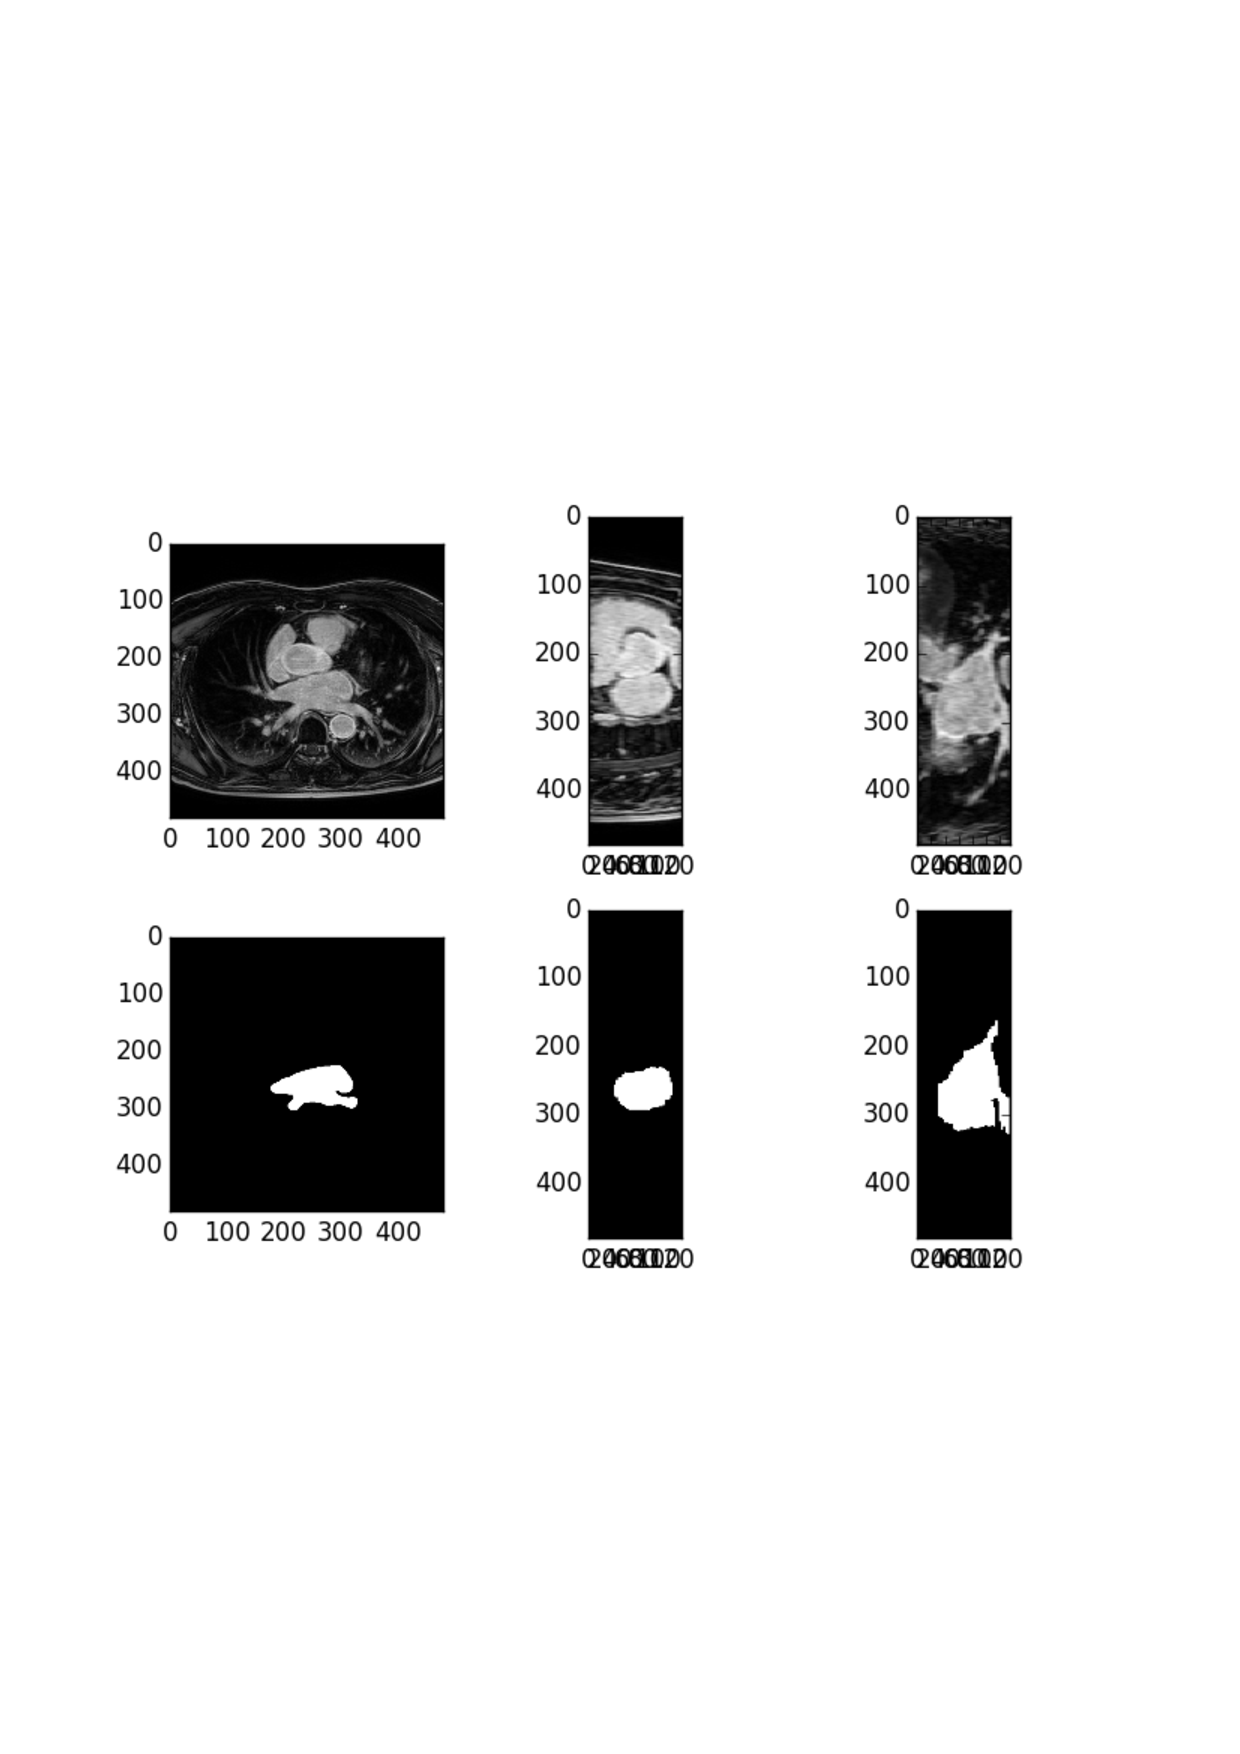
\includegraphics[trim=2cm 8cm 2cm 8cm, clip=true, height=60mm]{Chapter3/example_slice.pdf}
\end{minipage}\hfill
\begin{minipage}{0.45\textwidth}
\centering
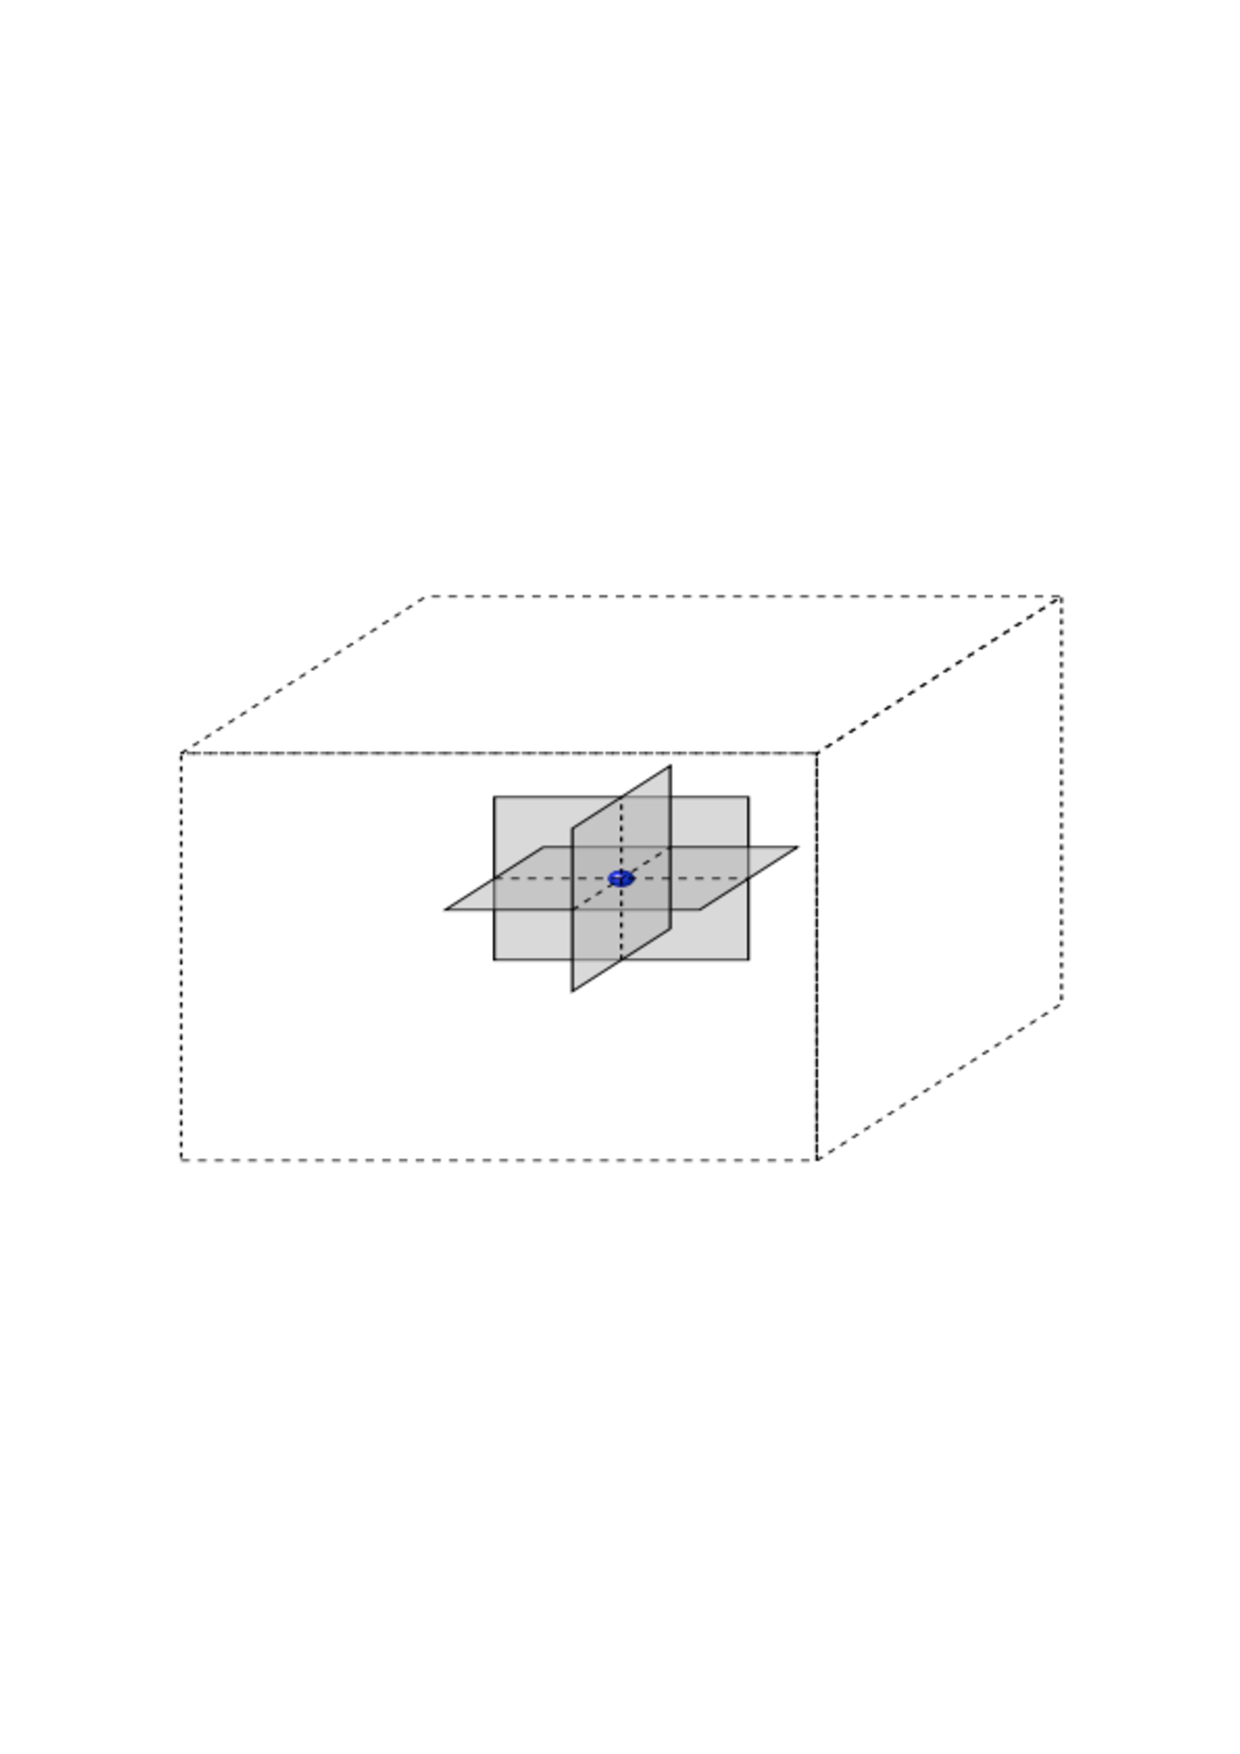
\includegraphics[trim=2cm 8cm 2cm 8cm, clip=true, height=60mm]{Chapter3/triplanar.pdf}
\end{minipage}
\caption{Left: grey scale slices from a CT scan taken in the transversal, saggital and coronal planes. Right: illustration of the triplanar}
\end{figure}

\section{Implementation Details}

\subsection{Libraries}

We use Torch, an open-source library maintained by Facebook in Lua aiming to provide a Matlab-like environment for scientific computing, along with a number of dependent libraries (cunn, cudnn, fbcunn) to train the convolutional networks on single and multi-GPUs. In addition, we use Python and a number of its libraries to handle all the logistics from generating the datasets to producing plots of segmentation results.

\subsection{Computer Power}

The training of the CNNs were conducted on 2 multi-GPU clusters, named montana-nvidia and montana-k80, kindly provided by Prof. Montana's laboratory. montana-nvidia consists 24 cores with 129 Gb of memory connected to two NVIDIA Tesla K40m and two Tesla K20Xm while montana-k80 on the other hand has 56 cores with 258 Gb of memory supported by 8 of NVIDIA's Testla K80. 

\section{Model Selection}

\subsection{General approach for model selection}

To look for a good model, we allocated 20 of the 27 CT scans to the training set, 7 to a testing set. We generated 400000 training examples equally divided among the training CT scans, half being in the atrium and the other half in the non-atrium part. The validation set is composed of 15000 testing examples from each testing CT scans to a total number of 105000 testing examples. The model selection is done by comparing the dice coefficient on the testing set calculated at the end of end epoch, which is just the classification accuracy in a 2-class problem, segmentation results from a few slices taken from the testing set and a final dice coefficient of the classification accuracy of the segmentation of the entire 7 testing CT scans preformed at the end of training.\\

We start off our model selection with a CNN composed of 2 convolutional layers with 32 and 64 feature maps respectively, 2 fully connected layers with 1000 and 500 hidden units each respectively, a logsoftmax output layer giving log probabilities. We will be varying in turn the following hyperparameters while keeping the rest constant.\\

\begin{itemize}
	\item varying the number of convolutional layers.
	\item varying the number of connected layers.
	\item varying the number of feature maps in the chosen number of convolutional layers.
	\item varying the number of hidden units in the chosen number of connected layers.
	\item varying the type of activation function (ReLU, Tanh or Sigmoid).
	\item varying the type of subsampling function (Maxpooling or average pooling).
	\item varying the learning rate.
	\item varying the momentum.
	\item varying the dataset size for the selected model.
\end{itemize}

\subsection{varying number of convolutional layers}

We start our model selection by the selecting the number of convolutional layers using four architectures with every other hyper parameter remaining the same. Their convolutional layers are given as

\begin{itemize}
	\item Input (6*32*32) => Conv layer (32*28*28) => 2*2 MaxPooling filter (32*14*14) 
	\item Input (6*32*32) => Conv layer (32*28*28) => 2*2 MaxPooling filter (32*14*14) => Conv layer (64*10*10) => 2*2 MaxPooling filter (64*5*5)
	\item Input (6*32*32) => Conv layer (32*28*28) => Conv layer (32*24*24) => 2*2 MaxPooling filter (32*12*12) => Conv layer (64*8*8) => 2*2 MaxPooling filter (64*4*4)
	\item Input (6*32*32) => Conv layer (32*28*28) => Conv layer (32*24*24) => 2*2 MaxPooling filter (32*12*12) => Conv layer (64*8*8) => Conv layer (64*4*4) => 2*2 MaxPooling filter (64*2*2)
\end{itemize}

These convolutional layers are then followed by two fully connected layers with 1000 and 500 hidden layers each. The following table gives the results for each of these architectures trained after 100 epochs.\\

\begin{tabular}{c|c|c|c|c|c}
\rowcolor[HTML]{C0C0C0} 
         & \begin{tabular}[c]{@{}c@{}}Dice \\ training set\end{tabular} & \begin{tabular}[c]{@{}c@{}}Dice \\ testing set\end{tabular} & Sensitivity & Specificity & \begin{tabular}[c]{@{}c@{}}Dice \\ test CT scan\end{tabular} \\ \hline
1 Conv L & 0.959                                                        & 0.956                                                       & 0.913       & 0.970       & 0.969                                                        \\ \hline
2 Conv L & 0.958                                                        & 0.961                                                       & 0.734       & 0.989       & 0.984                                                        \\ \hline
3 Conv L & 0.956                                                        & 0.960                                                       & 0.762       & 0.987       & 0.983                                                        \\ \hline
4 Conv L & 0.959                                                        & 0.956                                                       & 0.881       & 0.973       & 0.972                                                       
\end{tabular}\\

\noindent The dice coefficient over the training and testing sets are very similar while for the dice coefficient over the test CT scan, there is a significant improvement from 1 convolutional layer on the one hand to 2 and 3 on the other. This is explained by the increase specificity despite a significant drop in the sensitivity as the non-atrium voxels outnumber by a factor of almost 10 the number of atrium voxels. \\

\begin{figure}
\centering
\fbox{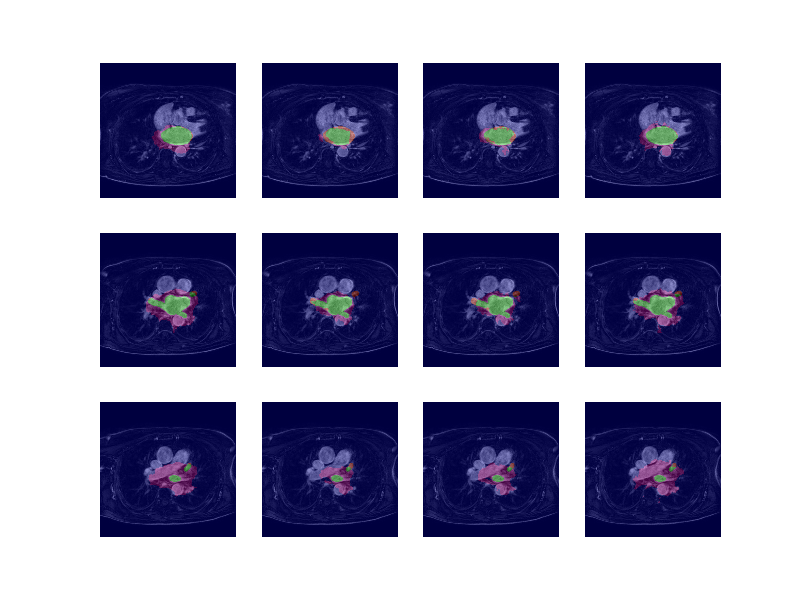
\includegraphics[trim=2cm 1cm 2cm 1cm, clip=true, height=80mm, width=150mm]{Chapter3/mask_results_varying_number_of_convolutional_layers.png}}
\caption{Left: grey scale slices from a CT scan taken in the transversal, saggital and coronal planes.}
\end{figure}

Figure whatever brings a visual element to this comparison. Each column shows the segmentation of a transversal slice of 3 different CT scan images. The first column corresponding to segmentations by the architecture with 1 convolutional layer as much larger pink patches, corresponding to false positives than the other two columns, corroborating the story told by the dice coefficients. There is not much difference between the masks of the second and third layers.\\

On that basis we choose to go with having 2 convolutional layers. 

\subsection{varying number of connected layers}

Having settled on an architecture with 2 convolutional layers, we now train 3 CNNs with 1, 2, and 3 fully connected layers each starting with 1000 hidden units and halving the number of hidden units for each additional layer. Hence the CNN with 3 fully connected layers has 1000, 500, and 250 hidden units in each respectively. Every other hyper parameter remain the same. The results are shown in the following table.\\

\begin{tabular}{c|c|c|c|c|c}
\rowcolor[HTML]{C0C0C0} 
              & \begin{tabular}[c]{@{}c@{}}Dice \\ training set\end{tabular} & \begin{tabular}[c]{@{}c@{}}Dice \\ testing set\end{tabular} & Sensitivity & Specificity & \begin{tabular}[c]{@{}c@{}}Dice \\ test CT scan\end{tabular} \\ \hline
1 Connected L & 0.957                                                        & 0.959                                                       & 0.887       & 0.972       & 0.971                                                        \\ \hline
2 Connected L & 0.958                                                        & 0.961                                                       & 0.856       & 0.974       & 0.972                                                        \\ \hline
3 Connected L & 0.953                                                        & 0.951                                                       & 0.915       & 0.967       & 0.966                                                       
\end{tabular}\\

The results for 1 and 2 fully connected layer architecture are very similar with very similar sensitivity and specificity and thus Dice coefficient for the test CT scan. However for 3 connected layers, there is a slight decrease in test CT scan dice coefficient from a comparatively lower specificity. Figure whatever shows very similar masks for the 1 and 2 connected layers and larger errors for the third column. 

\begin{figure}
\centering
\fbox{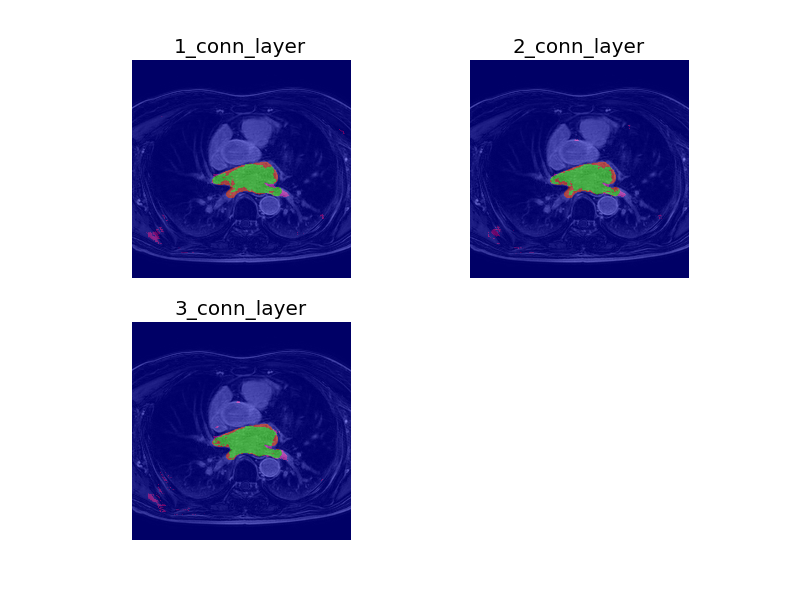
\includegraphics[trim=2cm 1cm 2cm 1cm, clip=true, height=80mm, width=150mm]{Chapter3/mask_results_varying_number_of_connected_layers.png}}
\caption{Left: grey scale slices from a CT scan taken in the transversal, saggital and coronal planes.}
\end{figure}

We choose to have 1 fully connected layer for our final architecture.

\subsection{varying number of feature maps}

So now the focus is on finding the right number of feature maps for the convolutional layers. In order to keep the computation comparable between the 2 layers, we set the number of feature maps in the second layer to be twice that of the first layer. We tried configurations with the first layer having 16, 32, 64, and 128 feature maps. The summary of the results are shown below.\\

\begin{tabular}{c|c|c|c|c|c}
\rowcolor[HTML]{C0C0C0} 
            & \begin{tabular}[c]{@{}c@{}}Dice \\ training set\end{tabular} & \begin{tabular}[c]{@{}c@{}}Dice \\ testing set\end{tabular} & Sensitivity & Specificity & \begin{tabular}[c]{@{}c@{}}Dice \\ test CT scan\end{tabular} \\ \hline
With 16 FM  & 0.956                                                        & 0.953                                                       & 0.919       & 0.967       & 0.966                                                        \\ \hline
With 32 FM  & 0.957                                                        & 0.958                                                       & 0.894       & 0.972       & 0.970                                                        \\ \hline
With 64 FM  & 0.959                                                        & 0.958                                                       & 0.904       & 0.971       & 0.970                                                        \\ \hline
With 128 FM & 0.962                                                        & 0.964                                                       & 0.875       & 0.976       & 0.974                                                       
\end{tabular}

There is not much difference between all four architectures. We thus settle with having a first layer with 16 feature maps.

\begin{figure}
\centering
\fbox{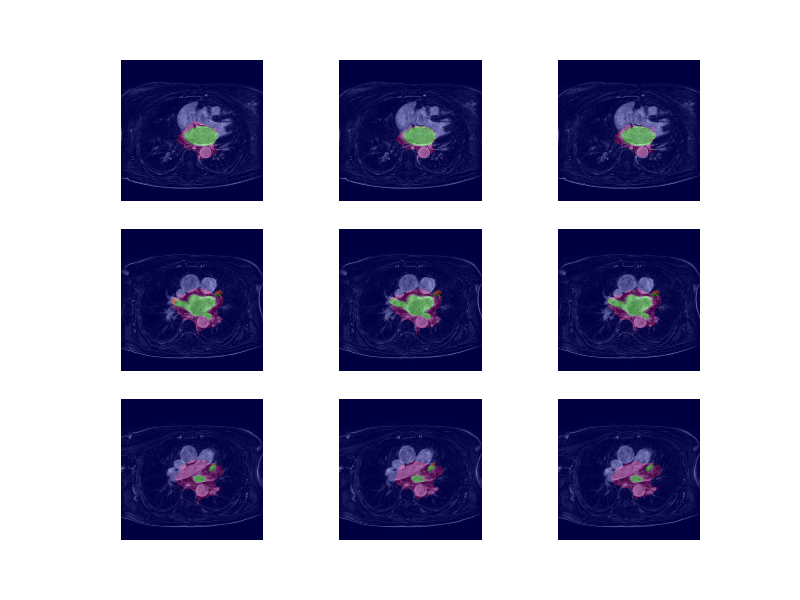
\includegraphics[trim=2cm 1cm 2cm 1cm, clip=true, height=80mm, width=150mm]{Chapter3/mask_results_varying_number_of_feature_maps.png}}
\caption{Left: grey scale slices from a CT scan taken in the transversal, saggital and coronal planes.}
\end{figure}

\subsection{varying the number of hidden units}

We now vary the number of hidden units in the connected layer, trying 100, 200, 500, 1000. 



\subsection{varying the activation function}

We experimented with different types of activation function: ReLU, Tanh, Sigmoid. Doing it with ReLU is better...




\subsection{varying the type of pooling}

We also tried different types of pooling: Max pooling and average pooling. No difference, so we stuck with Max pooling




\subsection{varying the learning rate}

Tried different learning rates: 0.01, 0.05, 0.1, 0.5, 1. It seems that 0.1 is best. Having a learning rate of 1 doesn't train the network.  We omitted the results.



\subsection{varying the momentum}

Tried different momentums: 0, 0.01, 0.05, 0.1. Having momentum actually slightly improves the test results!



\subsection{varying the data size}

Tried a number of dataset sizes: 400000, 1000000, 3000000: No improved result from the increased data size.

\subsection{varying datasets type}

The first thing we investigate is the sampling method for obtaining the training set. In order to increase the number of non-atrium training examples lying near the boundaries where we expect most of the classification errors to lie, we construct a rectangular area which contains the atrium. The atrium box is constructed by going through all the coordinates of the voxels labeled as being in the atrium, picking the minimum and maximum values in each of the coordinate planes, and possibly adding some padding, this procedure gives us a box containing the atrium. \\

We train our base CNN on 3 sampling procedures with no atrium box, i.e. all the non-atrium training examples are sampled randomly uniformly, a small atrium box constructed by the procedure above with a padding of 5 pixels in the x and y coordinate directions and of 1 pixel in the z coordinate direction, and finally a large atrium box with a padding of 30 pixels in the x and y coordinates and of 5 pixels in the z coordinate.\\

The results of the three training runs are shown in Figure whatever. From the testing dice coefficient plot, we get a better classification rate with sampling using an atrium box than no atrium box and particularly with the smaller atrium box. In the segmentation mask, sampling with no atrium box clearly yields more errors in the proximity of the atrium but none away from it whereas there are some errors far away from the atrium from the models trained with the atrium box sampling procedure. This is a consequence of the sampling procedures in both cases. Sampling with an atrium box would naturally yield better segmentation results near the atrium as the proportion of training examples is much higher in those regions than without an atrium box around it.\\




